\documentclass{standalone}
\usepackage{tikz}
\usetikzlibrary{patterns, positioning}


\begin{document}
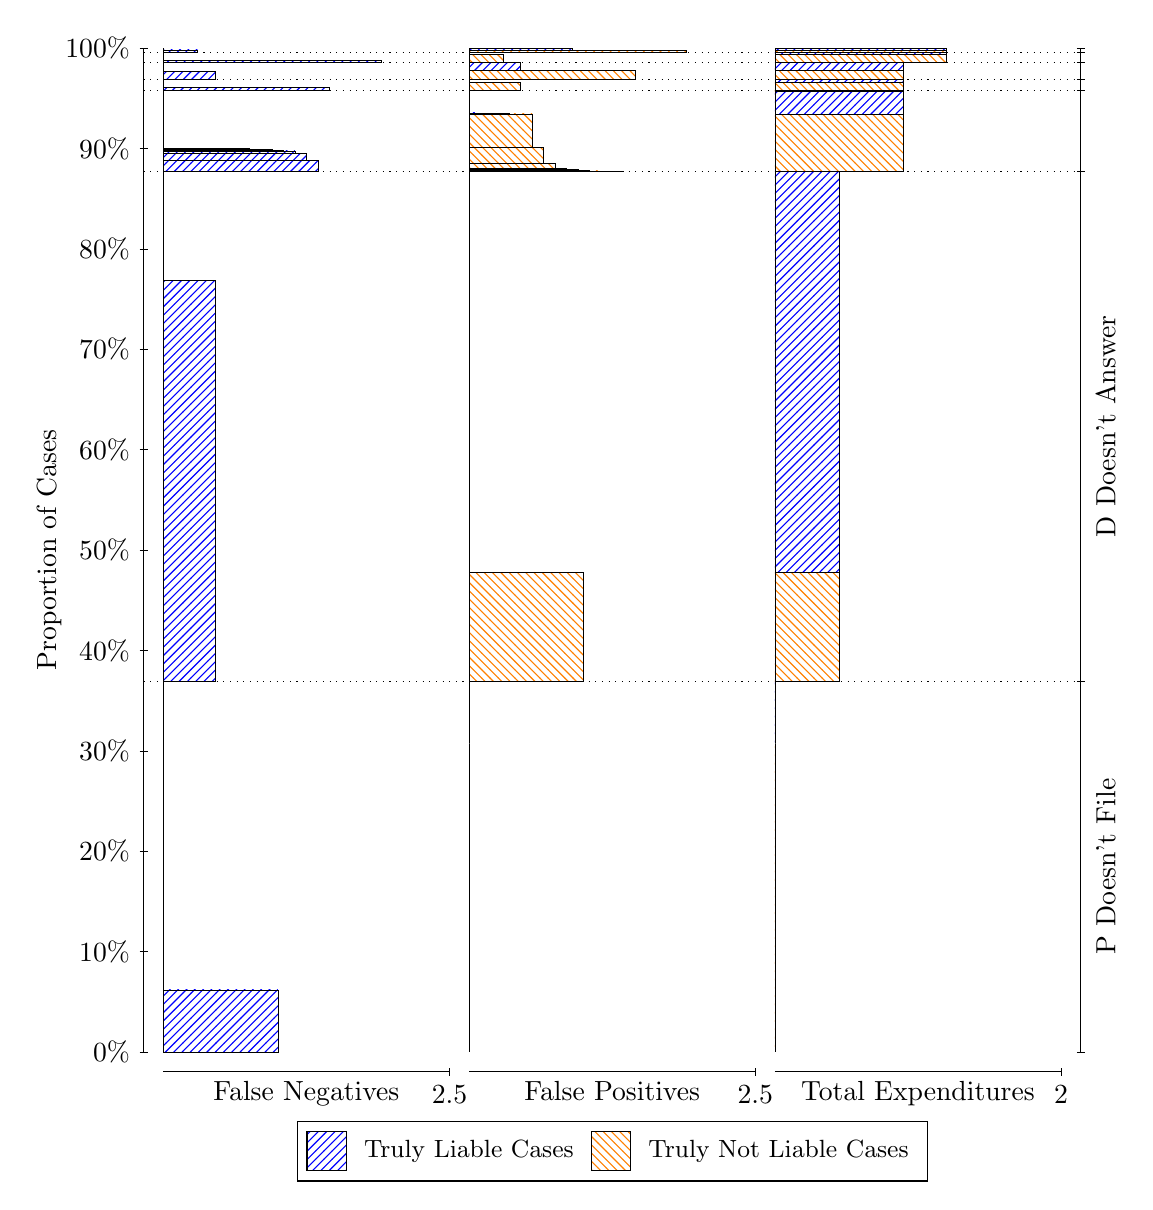
\begin{tikzpicture}
\draw[black, very thin] (1.5,1.75) -- (1.5,14.5);
\node[rotate=90, text=black, anchor=center] at (0.3, 8.125) {Proportion of Cases};
\draw[black, very thin] (1.45,1.75) -- (1.55,1.75);
\node[text=black, anchor=east] at (1.45, 1.75) {0\%};
\draw[black, very thin] (1.45,3.025) -- (1.55,3.025);
\node[text=black, anchor=east] at (1.45, 3.025) {10\%};
\draw[black, very thin] (1.45,4.3) -- (1.55,4.3);
\node[text=black, anchor=east] at (1.45, 4.3) {20\%};
\draw[black, very thin] (1.45,5.575) -- (1.55,5.575);
\node[text=black, anchor=east] at (1.45, 5.575) {30\%};
\draw[black, very thin] (1.45,6.85) -- (1.55,6.85);
\node[text=black, anchor=east] at (1.45, 6.85) {40\%};
\draw[black, very thin] (1.45,8.125) -- (1.55,8.125);
\node[text=black, anchor=east] at (1.45, 8.125) {50\%};
\draw[black, very thin] (1.45,9.4) -- (1.55,9.4);
\node[text=black, anchor=east] at (1.45, 9.4) {60\%};
\draw[black, very thin] (1.45,10.675) -- (1.55,10.675);
\node[text=black, anchor=east] at (1.45, 10.675) {70\%};
\draw[black, very thin] (1.45,11.95) -- (1.55,11.95);
\node[text=black, anchor=east] at (1.45, 11.95) {80\%};
\draw[black, very thin] (1.45,13.225) -- (1.55,13.225);
\node[text=black, anchor=east] at (1.45, 13.225) {90\%};
\draw[black, very thin] (1.45,14.5) -- (1.55,14.5);
\node[text=black, anchor=east] at (1.45, 14.5) {100\%};

\draw[black, very thin] (13.4,1.75) -- (13.4,14.5);
\draw[black, very thin] (13.35,1.75) -- (13.45,1.75);
\node[anchor=west] at (13.35, 1.75) {};
\draw[black, very thin] (13.35,6.4588) -- (13.45,6.4588);
\node[anchor=west] at (13.35, 6.4588) {};
\draw[black, very thin] (13.35,12.932) -- (13.45,12.932);
\node[anchor=west] at (13.35, 12.932) {};
\draw[black, very thin] (13.35,13.958) -- (13.45,13.958);
\node[anchor=west] at (13.35, 13.958) {};
\draw[black, very thin] (13.35,14.104) -- (13.45,14.104);
\node[anchor=west] at (13.35, 14.104) {};
\draw[black, very thin] (13.35,14.318) -- (13.45,14.318);
\node[anchor=west] at (13.35, 14.318) {};
\draw[black, very thin] (13.35,14.447) -- (13.45,14.447);
\node[anchor=west] at (13.35, 14.447) {};
\draw[black, very thin] (13.35,14.5) -- (13.45,14.5);
\node[anchor=west] at (13.35, 14.5) {};

\draw[black, very thin, pattern color=blue, pattern=north east lines] (1.75,1.75) rectangle (3.2033,2.5394);
\draw[black, very thin, pattern color=orange, pattern=north west lines] (1.75,2.5394) rectangle (1.75,6.4588);
\draw[black, very thin, pattern color=blue, pattern=north east lines] (1.75,6.4588) rectangle (2.404,11.55);
\draw[black, very thin, pattern color=orange, pattern=north west lines] (1.75,11.55) rectangle (1.75,12.932);
\draw[black, very thin, pattern color=blue, pattern=north east lines] (1.75,12.932) rectangle (3.712,13.069);
\draw[black, very thin, pattern color=blue, pattern=north east lines] (1.75,13.069) rectangle (3.5667,13.161);
\draw[black, very thin, pattern color=blue, pattern=north east lines] (1.75,13.161) rectangle (3.4213,13.193);
\draw[black, very thin, pattern color=blue, pattern=north east lines] (1.75,13.193) rectangle (3.276,13.201);
\draw[black, very thin, pattern color=blue, pattern=north east lines] (1.75,13.201) rectangle (3.276,13.203);
\draw[black, very thin, pattern color=blue, pattern=north east lines] (1.75,13.203) rectangle (3.1307,13.213);
\draw[black, very thin, pattern color=blue, pattern=north east lines] (1.75,13.213) rectangle (2.9853,13.216);
\draw[black, very thin, pattern color=blue, pattern=north east lines] (1.75,13.216) rectangle (2.84,13.221);
\draw[black, very thin, pattern color=blue, pattern=north east lines] (1.75,13.221) rectangle (2.6947,13.224);
\draw[black, very thin, pattern color=blue, pattern=north east lines] (1.75,13.224) rectangle (2.5493,13.226);
\draw[black, very thin, pattern color=orange, pattern=north west lines] (1.75,13.226) rectangle (1.75,13.958);
\draw[black, very thin, pattern color=blue, pattern=north east lines] (1.75,13.958) rectangle (3.8573,14.002);
\draw[black, very thin, pattern color=orange, pattern=north west lines] (1.75,14.002) rectangle (1.75,14.104);
\draw[black, very thin, pattern color=blue, pattern=north east lines] (1.75,14.104) rectangle (2.404,14.207);
\draw[black, very thin, pattern color=orange, pattern=north west lines] (1.75,14.207) rectangle (1.75,14.318);
\draw[black, very thin, pattern color=blue, pattern=north east lines] (1.75,14.318) rectangle (4.5113,14.342);
\draw[black, very thin, pattern color=orange, pattern=north west lines] (1.75,14.342) rectangle (1.75,14.447);
\draw[black, very thin, pattern color=blue, pattern=north east lines] (1.75,14.447) rectangle (2.186,14.477);
\draw[black, very thin, pattern color=orange, pattern=north west lines] (1.75,14.477) rectangle (1.75,14.5);
\draw[black, very thin, pattern color=orange, pattern=north west lines] (5.6333,1.75) rectangle (5.6333,5.6693);
\draw[black, very thin, pattern color=blue, pattern=north east lines] (5.6333,5.6693) rectangle (5.6333,6.4588);
\draw[black, very thin, pattern color=orange, pattern=north west lines] (5.6333,6.4588) rectangle (7.0867,7.8404);
\draw[black, very thin, pattern color=blue, pattern=north east lines] (5.6333,7.8404) rectangle (5.6333,12.932);
\draw[black, very thin, pattern color=orange, pattern=north west lines] (5.6333,12.932) rectangle (7.5953,12.933);
\draw[black, very thin, pattern color=orange, pattern=north west lines] (5.6333,12.933) rectangle (7.45,12.935);
\draw[black, very thin, pattern color=orange, pattern=north west lines] (5.6333,12.935) rectangle (7.3047,12.939);
\draw[black, very thin, pattern color=orange, pattern=north west lines] (5.6333,12.939) rectangle (7.1593,12.943);
\draw[black, very thin, pattern color=orange, pattern=north west lines] (5.6333,12.943) rectangle (7.014,12.957);
\draw[black, very thin, pattern color=orange, pattern=north west lines] (5.6333,12.957) rectangle (6.8687,12.96);
\draw[black, very thin, pattern color=orange, pattern=north west lines] (5.6333,12.96) rectangle (6.8687,12.974);
\draw[black, very thin, pattern color=orange, pattern=north west lines] (5.6333,12.974) rectangle (6.7233,13.035);
\draw[black, very thin, pattern color=orange, pattern=north west lines] (5.6333,13.035) rectangle (6.578,13.239);
\draw[black, very thin, pattern color=orange, pattern=north west lines] (5.6333,13.239) rectangle (6.4327,13.664);
\draw[black, very thin, pattern color=blue, pattern=north east lines] (5.6333,13.664) rectangle (6.142,13.666);
\draw[black, very thin, pattern color=blue, pattern=north east lines] (5.6333,13.666) rectangle (5.9967,13.669);
\draw[black, very thin, pattern color=blue, pattern=north east lines] (5.6333,13.669) rectangle (5.8513,13.674);
\draw[black, very thin, pattern color=blue, pattern=north east lines] (5.6333,13.674) rectangle (5.706,13.677);
\draw[black, very thin, pattern color=blue, pattern=north east lines] (5.6333,13.677) rectangle (5.6333,13.958);
\draw[black, very thin, pattern color=orange, pattern=north west lines] (5.6333,13.958) rectangle (6.2873,14.06);
\draw[black, very thin, pattern color=blue, pattern=north east lines] (5.6333,14.06) rectangle (5.6333,14.104);
\draw[black, very thin, pattern color=orange, pattern=north west lines] (5.6333,14.104) rectangle (7.7407,14.216);
\draw[black, very thin, pattern color=blue, pattern=north east lines] (5.6333,14.216) rectangle (6.2873,14.318);
\draw[black, very thin, pattern color=orange, pattern=north west lines] (5.6333,14.318) rectangle (6.0693,14.424);
\draw[black, very thin, pattern color=blue, pattern=north east lines] (5.6333,14.424) rectangle (5.6333,14.447);
\draw[black, very thin, pattern color=orange, pattern=north west lines] (5.6333,14.447) rectangle (8.3947,14.47);
\draw[black, very thin, pattern color=blue, pattern=north east lines] (5.6333,14.47) rectangle (6.9413,14.5);
\draw[black, very thin, pattern color=orange, pattern=north west lines] (9.5167,1.75) rectangle (9.5167,5.6693);
\draw[black, very thin, pattern color=blue, pattern=north east lines] (9.5167,5.6693) rectangle (9.5167,6.4588);
\draw[black, very thin, pattern color=orange, pattern=north west lines] (9.5167,6.4588) rectangle (10.334,7.8404);
\draw[black, very thin, pattern color=blue, pattern=north east lines] (9.5167,7.8404) rectangle (10.334,12.932);
\draw[black, very thin, pattern color=orange, pattern=north west lines] (9.5167,12.932) rectangle (11.152,12.933);
\draw[black, very thin, pattern color=blue, pattern=north east lines] (9.5167,12.933) rectangle (11.152,12.935);
\draw[black, very thin, pattern color=orange, pattern=north west lines] (9.5167,12.935) rectangle (11.152,13.662);
\draw[black, very thin, pattern color=blue, pattern=north east lines] (9.5167,13.662) rectangle (11.152,13.951);
\draw[black, very thin, pattern color=orange, pattern=north west lines] (9.5167,13.951) rectangle (11.152,13.955);
\draw[black, very thin, pattern color=blue, pattern=north east lines] (9.5167,13.955) rectangle (11.152,13.958);
\draw[black, very thin, pattern color=orange, pattern=north west lines] (9.5167,13.958) rectangle (11.152,14.06);
\draw[black, very thin, pattern color=blue, pattern=north east lines] (9.5167,14.06) rectangle (11.152,14.104);
\draw[black, very thin, pattern color=orange, pattern=north west lines] (9.5167,14.104) rectangle (11.152,14.216);
\draw[black, very thin, pattern color=blue, pattern=north east lines] (9.5167,14.216) rectangle (11.152,14.318);
\draw[black, very thin, pattern color=orange, pattern=north west lines] (9.5167,14.318) rectangle (11.697,14.424);
\draw[black, very thin, pattern color=blue, pattern=north east lines] (9.5167,14.424) rectangle (11.697,14.447);
\draw[black, very thin, pattern color=orange, pattern=north west lines] (9.5167,14.447) rectangle (11.697,14.47);
\draw[black, very thin, pattern color=blue, pattern=north east lines] (9.5167,14.47) rectangle (11.697,14.5);
\draw[black, dotted] (1.5,6.4588) -- (13.4,6.4588);
\draw[black, dotted] (1.5,12.932) -- (13.4,12.932);
\draw[black, dotted] (1.5,13.958) -- (13.4,13.958);
\draw[black, dotted] (1.5,14.104) -- (13.4,14.104);
\draw[black, dotted] (1.5,14.318) -- (13.4,14.318);
\draw[black, dotted] (1.5,14.447) -- (13.4,14.447);
\draw[black, very thin] (1.75,1.5) -- (5.3833,1.5);
\node[text=black, anchor=north] at (3.5667, 1.5) {False Negatives};
\draw[black, very thin] (5.3833,1.45) -- (5.3833,1.55);
\node[text=black, anchor=north] at (5.3833, 1.45) {2.5};

\draw[black, very thin] (5.6333,1.5) -- (9.2667,1.5);
\node[text=black, anchor=north] at (7.45, 1.5) {False Positives};
\draw[black, very thin] (9.2667,1.45) -- (9.2667,1.55);
\node[text=black, anchor=north] at (9.2667, 1.45) {2.5};

\draw[black, very thin] (9.5167,1.5) -- (13.15,1.5);
\node[text=black, anchor=north] at (11.333, 1.5) {Total Expenditures};
\draw[black, very thin] (13.15,1.45) -- (13.15,1.55);
\node[text=black, anchor=north] at (13.15, 1.45) {2};

\node[text=black, centered, rotate=90] at (13.72, 4.1044) {P Doesn't File};
\node[text=black, centered, rotate=90] at (13.72, 9.6953) {D Doesn't Answer};






\draw (7.449999999999999,1.5) node[draw=none] (baseCoordinate) {};
\begin{scope}[align=center]
        \matrix[scale=0.5, draw=black, below=0.5cm of baseCoordinate, nodes={draw}, column sep=0.1cm]{
            \node[rectangle, draw, minimum width=0.5cm, minimum height=0.5cm, pattern color=blue, pattern=north east lines] {}; &
            \node[draw=none, font=\small, text=black] (B) {Truly Liable Cases}; &
            \node[rectangle, draw, minimum width=0.5cm, minimum height=0.5cm, pattern color=orange, pattern=north west lines] {}; &
            \node[draw=none, font=\small, text=black] (B) {Truly Not Liable Cases}; \\
            };
\end{scope}

\end{tikzpicture}
\end{document}